% Bla bla bla ...

% % \begin{figure}
%     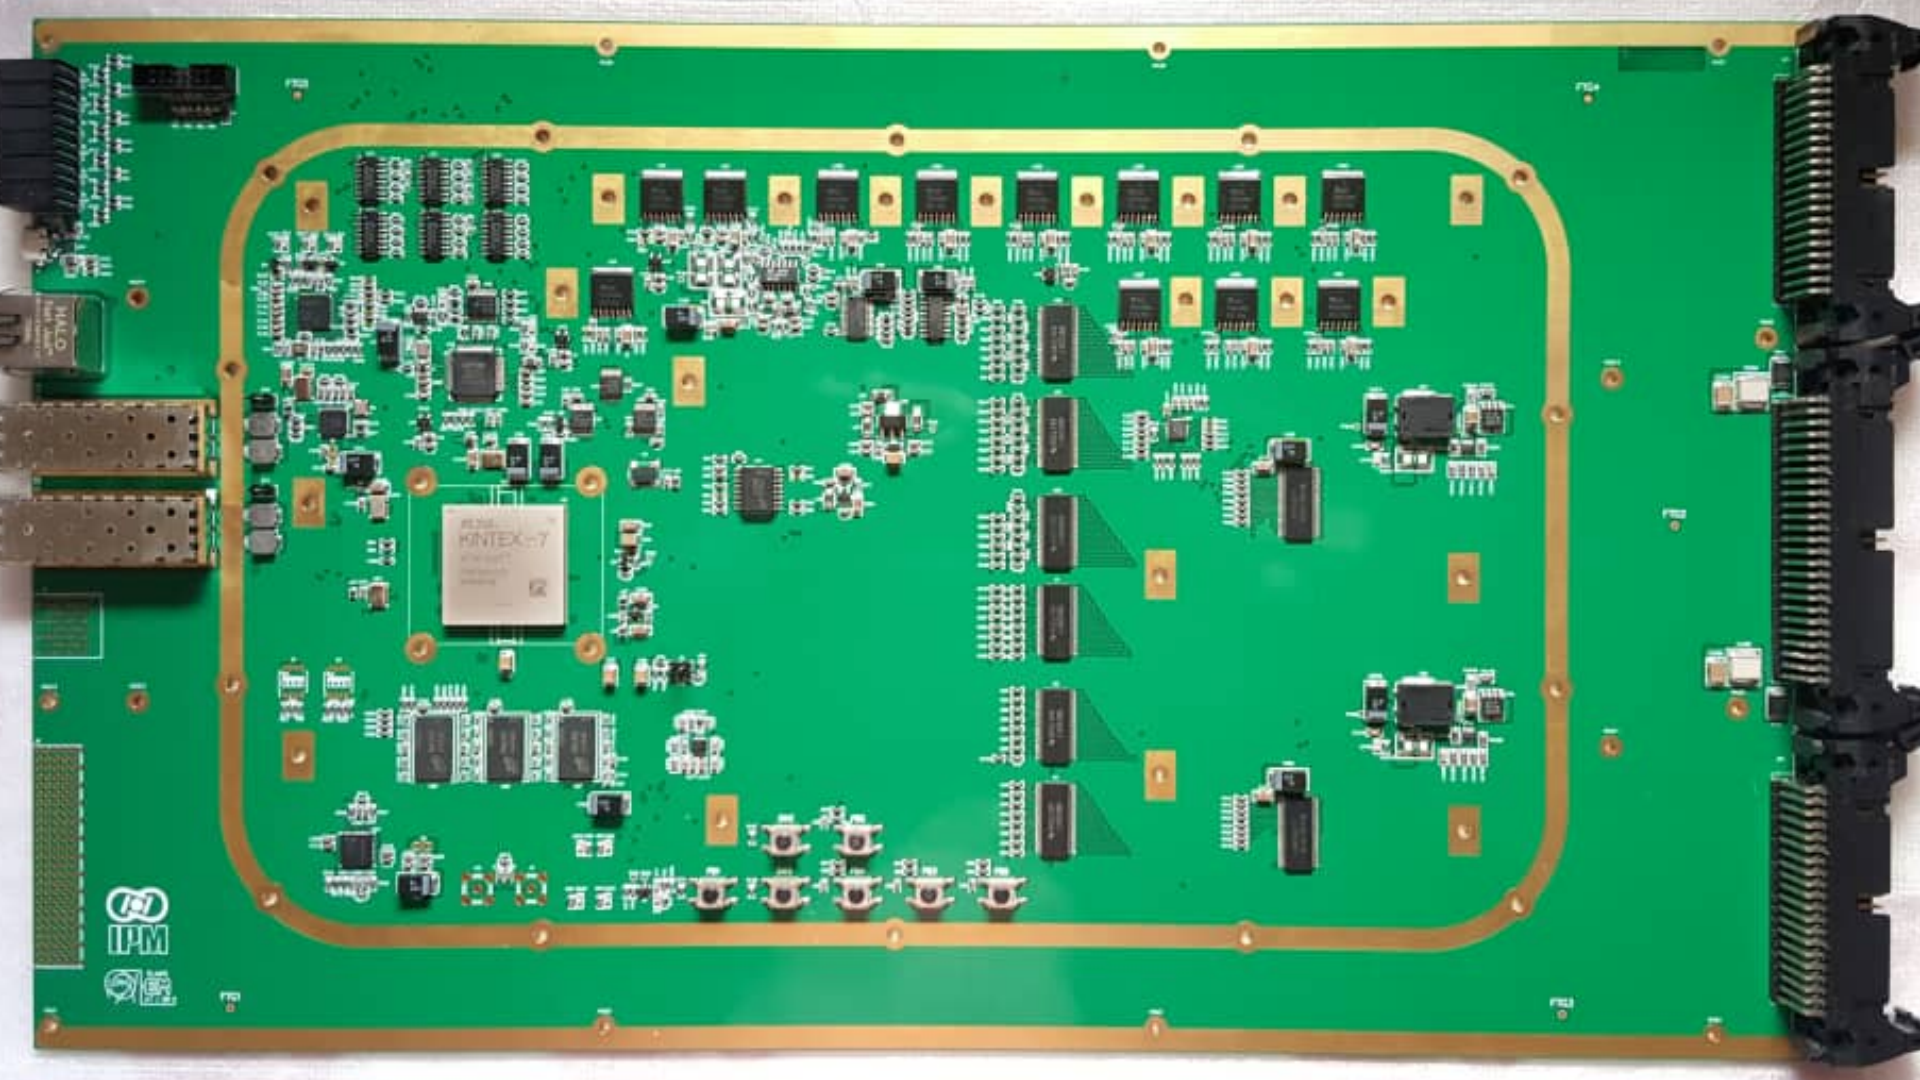
\includegraphics[width=1\textwidth]{uioposter-images/link_system_board}
%     % \caption{\footnotesize A quadrant of the CMS Muon Spectrometer, showing DT chambers (yellow), RPCs (light blue), and CSCs (green). The locations of new forward muon detectors for the HL-LHC project are contained within the dashed box and indicated in red for Gas Electron Multiplier (GEM) stations (ME0, GE1/1, and GE2/1) and violet for improved RPC stations (RE3/1 and RE4/1).}
% %     \label{cms_muon_upgrade}
% % \end{figure}

% Bla bla bla ...



In the CMS experiment, the RPC chambers are readout, controlled and monitored through the Link System, which consists of 1592 electronics boards, divided in two kinds, known as the Link boards (LBs) and Control Boards (CBs), LBs can work as Master LB or Slave LB.  

% Details of the CMS RPC readout and control are shown in Figure~\ref{rpc_phase2_readout}.

\begin{wrapfigure}[6]{r}{0.5\textwidth}
    % \hskip1cm
    \caption{\footnotesize A RPC Link Board prototype for Phase-2 Upgrade.}
    \label{link_system}.
    % \hfill
    % \center
    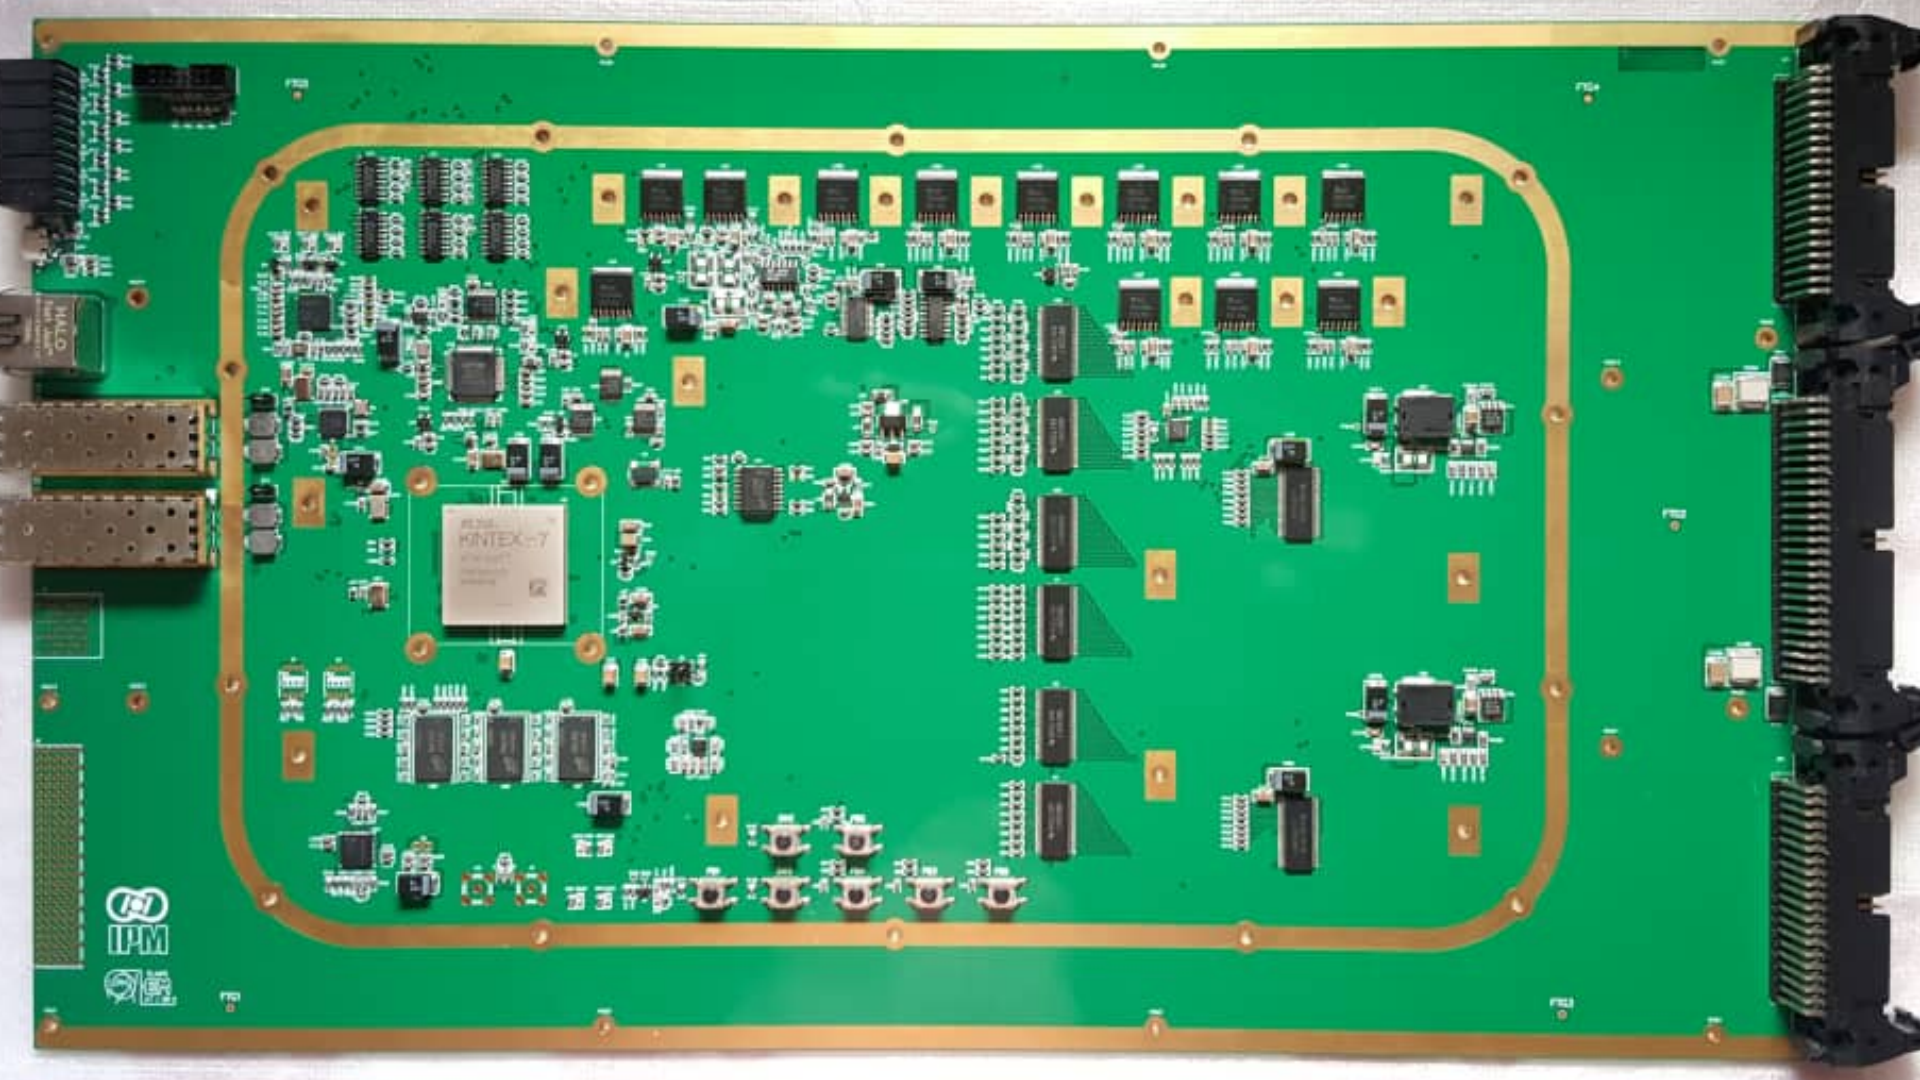
\includegraphics[width=0.49\textwidth]{uioposter-images/link_system_board.png}
\end{wrapfigure}

% The HL-LHC high rates will required an increase of the available TX bandwidth and readout time resolution. 

The new link system is being developed around the use of modern components and FPGAs (Field Programmable Gate Array), following a radiation hard design. 

\begin{tcolorbox}[colback=gray!5,colframe=gray!40!black]
    \textbf{The data transmission rate between the new Link system and RPC back-end electronics increases to 10.24 Gbps and resolution of the Muon hit time improves to 1.5 ns.}
\end{tcolorbox}

% \textbf{}

\hfill

This is achieved by \textbf{(1) the use GTX transceivers of the FPGA}, plus preprocessing of data and (2) implementing a high resolution \textbf{96-channel Time-to-Digital Converter (TDC) in the link board FPGA}. Each TDC channel comprised of 16 bins where each bin had a time scale of 25/16 ns. The experimental results showed that there existed a 1.56 ns resolution for the implemented TDC channels. 

% The high speed data transmissions is obtained by the use of a GTX transceivers of the FPGA, plus preprocessing of data before sending to the GTX transmitter.






